\section[The inverse function theorem]{The inverse function theorem}
\paragraph{Motivation}
In analysis of functions of one variable we had that
\begin{thm}
Given
\begin{enumerate}
\item $f: I \rightarrow \RR.\ I \subset \RR$ ($I$ being an open interval)
\item $f$ is continuously differentiable on its domain (interval $I$)
\item $f'(x) \neq 0\  \forall x \in I$ (i.e. $f$ is strictly increasing or decreasing)
\end{enumerate}
Then $f$ is invertible (bijective), its inverse $f^{-1}$ is also continuously differentiable and
$$(f^{-1})'(f(x)) = \frac{1}{f'(x)}$$
\end{thm}

\begin{rem}
  Can be derived as $$f^{-1}(f(x)) = x\ \underrightarrow{^\text{differentiate}}\ (f^{-1})'(f(x)).f'(x) = 1 \iff (f^{-1})'(f(x)) = \frac{1}{f'(x)}$$
  \end{rem}

\begin{figure}[hb]
  \center
\caption{Geometric idea of inverse function theorem}
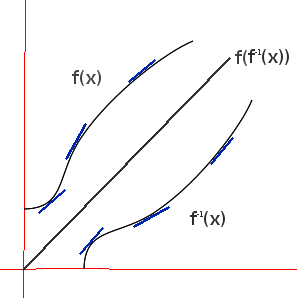
\includegraphics[scale=0.6]{figures/invfuncthm}
\end{figure}

We wish to generalize this statement to functions of multiple variables.
\begin{ldefn}
  We call $f|_u$ a restriction of $f$ at $u$; we only consider $f$ on the sub-domain $u$ and its image from $u$.
\end{ldefn}

\begin{thm}[Inverse function theorem for functions of several variables]
  Given
  \begin{enumerate}
  \item $f: u \rightarrow \RR^n. u \subset \RR^n$ ($u$ is an open n-ball)
  \item $f$ is differentiable on $u$, or, equivalently, $f|_u$ is differentiable
  \item $Df: u \rightarrow L(\RR^n)$ is continuous.
  \item $Df(x_0)$ is invertible $x_0 \in u$, or, equivalently, that the jacobean $J_f(x_0)$ is invertible in $M^{n\times n}$
  \end{enumerate}
  Then $\exists$ neighbohrhood $u_0 \subset u$ of $x_0$ so that $f|_{u_0}$ is bijective onto its image $v_0 = f(u_0)$ (invertible), the inverse $g = (f|_{u_0})^{-1}$ is also differentiable on $v_0$ and $\forall y = f(x) \in v_0$
  $$Dg(y) = (Df(x))^{-1}$$
  or, equivalently
  $$J_g(y) = (J_f(x))^{-1}$$
\end{thm}

Proof sketch:
\begin{enumerate}[I]
\item $\exists u_0$ neighbourhood of $x_0$ such that $f|_{u_0}$ is bijective with inverse $g: v_0 \rightarrow u_0$, where $v_0 = f(u_0)$ (using \emph{Banach fixed point theorem}
\item $v_0$ is open
\item $g$ is differentiable on $v_0$ and $D_g(y) = (Df(g(y)))^{-1}, \forall y \in v_0$
\end{enumerate}

\begin{defn}
  A function defined from metric space $(\Set{X}, d)$ to itself $\kappa: \Set{X} \rightarrow \Set{X}$ is called a contraction if
  $$d(\kappa(x), \kappa(y)) < cd(x,y).\ \forall x, y \in \Set{X}.\ c \in [0, 1)$$
\end{defn}

\begin{rem}
  Intuitive picture of a contraction $\kappa$ involves  a function where the preimage always changes faster than the image; graph would be `flatter' the smaller $c$ is.
\end{rem}

\begin{ldefn}
  A complete metric space is a metric space where all cauchy sequences converge. i.e. $$((x_p) \in \Set{X} \implies \forall \epsilon > 0 . \ \exists N_\epsilon \in \NN : d(x_p, x_q) < \epsilon .\  \forall p, q \geq N_\epsilon) \implies x_p \underrightarrow{^{p\rightarrow \infty}} x \in \Set{X} $$
\end{ldefn}

\begin{thm}[Banach fixed point theorem]
  Let $(\Set{X}, d)$ be a complete metric space. If $\kappa: \Set{X} \rightarrow \Set{X}$ is a contraction mapping, then $\kappa$ has a unique fixed point $x \in \Set{X}$, i.e. a point $x \in \Set{X}$ where $\kappa(x) = x$.
\end{thm}

\begin{rem}
  Intuitive picture of Banach fixed point theorem: because $\kappa$ is a contraction (the preimage $x$ is always changing faster than the image $\kappa(x)$), you know that somewhere as you're moving towards either its maximal point (e.g: $+\infty$) or minimal point (e.g: $-\infty$) the value of $x$ will catch up to $\kappa(x)$
\end{rem}

\begin{proof}
  \begin{enumerate}
  \item Take some $x_1 \in \Set{X}$
  \item Define sequence $(x_p)$ inductively such that $x_{p+1} = \kappa^p(x_1).\ p \in \NN$
  \item Define inequality
    $$d(x_{p+1}, x_p) \leq c^{p-1}d(x_2, x_1).\ p \in \NN.\ c \in [0, 1) \:\:\:\: \text{*}$$ 
    where $c$ is the contraction constant for $\kappa$. 
  \item Proving above inequality by induction.
    \par Base case (p = k = 1):
    $$d(x_{1+1}, x_1) \leq c^{1-1}d(x_2, x_1)$$
    $$d(x_2, x_1) \leq (c^0)d(x_2, x_1) \implies d(x_2, x_1) = d(x_2, x_1)$$
    \par Inductive step (p = k + 1)
    $$d(x_{k+2}, x_{k+1}) = d(\kappa(x_{k+1}), \kappa(x_{k}))$$
    Since $\kappa$ is a contraction
    $$ = d(\kappa(x_{k+1}), \kappa(x_k)) \leq cd(x_{k+1}, x_k)$$
    Activate induction
    $$ \leq cc^{k-1}d(x_2, x_1) = c^kd(x_2, x_1)$$
  \item We will show the sequence $(x_p)$ is cauchy. Let $m, n \in \NN.\ m > n$
  \item By triangle inequality
    $$d(x_m, x_n) \leq d(x_m, x_{m-1}) + d(x_{m-1}, x_{m-2}) + \dots + d(x_{n+1}, x_n)$$
    By inequality (*)
    $$\phantom{d(x_m, x_n) } \leq c^{m-2}d(x_2, x_1)+c^{m-3}d(x_2, x_1)+\dots + c^{n-1}d(x_2, x_1)$$
    $$\phantom{d(x_m, x_n) } = c^{n-1}d(x_2, x_1)\sum_{k=0}^{m-n-2}c^k$$
    $$\phantom{d(x_m, x_n) } \leq c^{n-1}d(x_2, x_1)\sum_{k=0}^{\infty}c^k = c^{n-1}d(x_2, x_1)\frac{1}{1-c}$$
    So finally
    $$d(x_m, x_n) = c^{n-1}\frac{d(x_2, x_1)}{1-c}$$
  \item Let $\epsilon = c^{N-1}\frac{d(x_2, x_1)}{1-c} > 0 \iff N = \lceil \log_c(\frac{\epsilon(1-c)}{d(x_2, x_1)})\rceil + 1$
  \item $\epsilon$ is arbitrary, so the sequence $(x_p)$ is cauchy. And since the metric space it is defined on, $(\Set{X}, d)$, is complete, it converges to some $x^* \in \Set{X}$.
  \item $\kappa$ is a contraction $\implies$ Lipschitz (with constant $< 1$) $\iff$ Lipschitz continuous. Thus we can have
    $$\kappa(\lim_{p\rightarrow \infty}x_p) = \lim_{p\rightarrow \infty}x_{p+1}$$
    $$\kappa(x^*) = x^*$$
    So $x^*$ is a fixed point of $\kappa$
  \item Suppose there exists another $y \in \Set{X}$ such that $\kappa(y) = y$, then
    $$0 \leq d(x^*, y) = d(\kappa(x^*), \kappa(y)) \leq cd(x^*, y)$$
    Since $|c| < 1$, $d(x^*, y) = 0$
    $$0 \leq d(\kappa(x^*), \kappa(y)) \leq 0$$
    $$x^* = \kappa(x^*) = \kappa(y) = y$$
    So $x^*$ is the unique fixed point.
  \end{enumerate}
\end{proof}

